
\documentclass[11pt, letter]{article} 

\usepackage[english]{babel}
\usepackage{booktabs} 
\usepackage{comment} 
\usepackage[utf8]{inputenc}
\usepackage[T1]{fontenc}


\usepackage{amsmath,amsfonts,amsthm} 
\usepackage{tikz}
\usepackage{tikz-cd}
\usepackage{systeme}
\usetikzlibrary{positioning,arrows}
\usetikzlibrary{decorations.pathreplacing}
\usepackage{tikzsymbols}
\usepackage{blindtext} 
\newcommand\scalemath[2]{\scalebox{#1}{\mbox{\ensuremath{\displaystyle #2}}}}

\usepackage{geometry}

\geometry{
	top=2cm, 
	bottom=2cm, 
	left=2.2cm, 
	right=2.2cm, 
	includehead
}

\setlength{\parindent}{15pt} 
\usepackage{setspace}
% Two options:
\linespread{1.5}

\usepackage[T1]{fontenc} 
\usepackage[utf8]{inputenc} 

\usepackage{XCharter}
\usepackage{tikz}
\usetikzlibrary{arrows}
\usepackage{graphicx}
\usepackage[export]{adjustbox}
\usepackage{subcaption}



\usepackage{fancyhdr} 
\pagestyle{fancy} 

\lhead{} 
\chead{\textit{}} 
\rhead{} 


\lfoot{} 
\cfoot{\footnotesize \thepage} 
\rfoot{ } 


\usepackage{biblatex}
\addbibresource{literature.bib}
\usepackage[style=numeric]{biblatex}




\newcommand{\signature}[2][5cm]{%
  \begin{tabular}{@{}p{#1}@{}}
    #2 \\[2\normalbaselineskip] \hrule \\[0pt]
    {\small \textit{Signature}} \\[2\normalbaselineskip] \hrule \\[0pt]
    {\small \textit{Place, Date}}
  \end{tabular}
}

\title{Exploratory Visualization Deliverable}
\author{Jashwanth Sompalli, Charlie Shaw, Stephen Tan, Justin Wong}

\date{ \small DATASCI W209 - Fall 2022}
\begin{document}

\maketitle 

\begin{center}
 

\end{center}

\setcounter{page}{1}

\section*{Hypothesis 1}
\noindent Increases in state-wide temperatures from 1960 to 2020 correlates with more hurricanes across the United States.
\subsection*{Iteration 1}

\begin{figure}[h!]
    \centering
    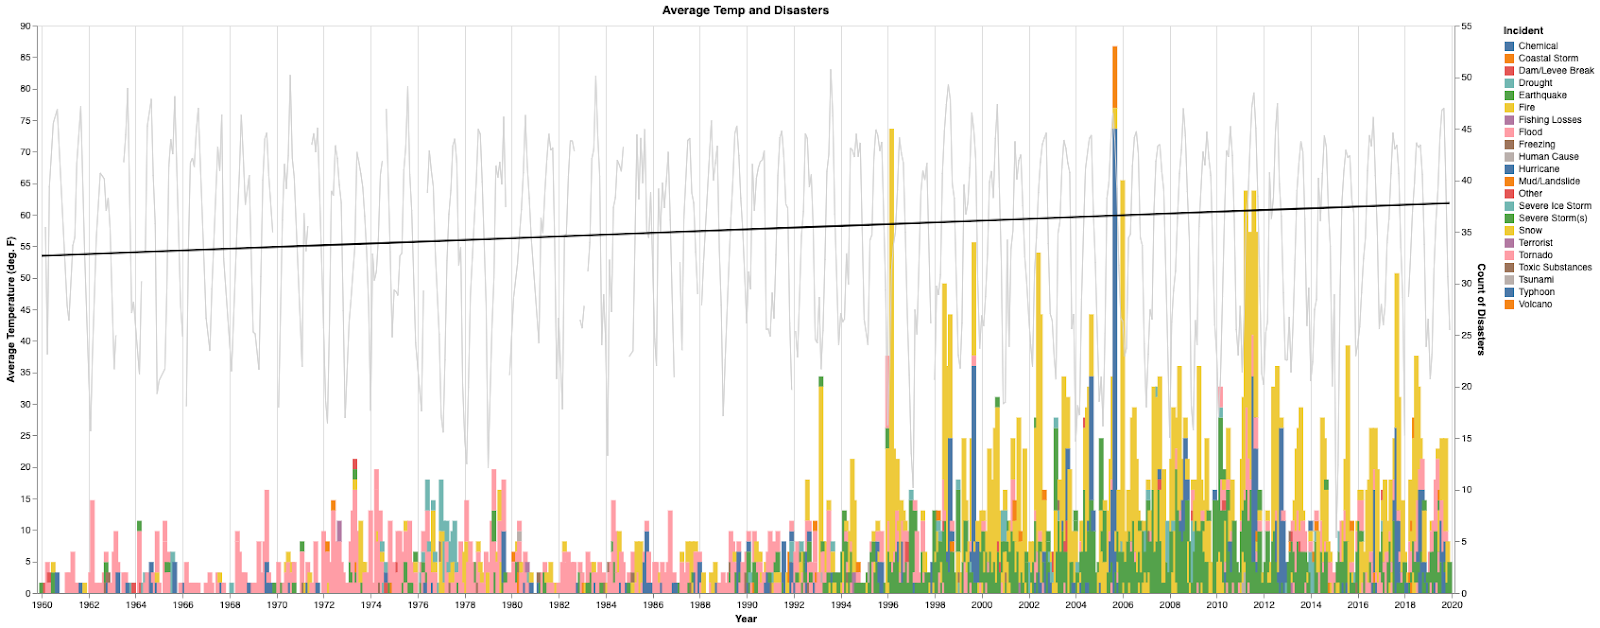
\includegraphics[scale=0.3]{iter1_h1.png}
    \caption{Hypothesis 1 - Iteration 1}
    \label{fig:my_label}
\end{figure}

\subsubsection*{What is Informative About This View?}
This view shows time series data between 1960–2020. On the x-axis, the year range is shown. For the y-axes, there is an axis on the left that includes the average temperature in Fahrenheit and another axis on the right that shows the count of all incidents recorded in each year. A best fit line through the average monthly temperatures shows that temperature has been steadily increasing. This view is helpful in understanding how more incidents are correlated with a rise in temperature.
\subsubsection*{What Could Be Improved About This View?}
 Since there are so many incident categories, the visualization looks messy. It is clear that pink, green, and yellow are the most common incidents, which correspond to flood, fire, and severe storm, respectively. However, there is cognitive load on the viewer, and it is difficult to match the color to the legend on the right. For example, flood and tornado are both designated as shades of pink, but it is difficult to discern them apart. 

\subsection*{Iteration 2}
\begin{figure}[h!]
    \centering
    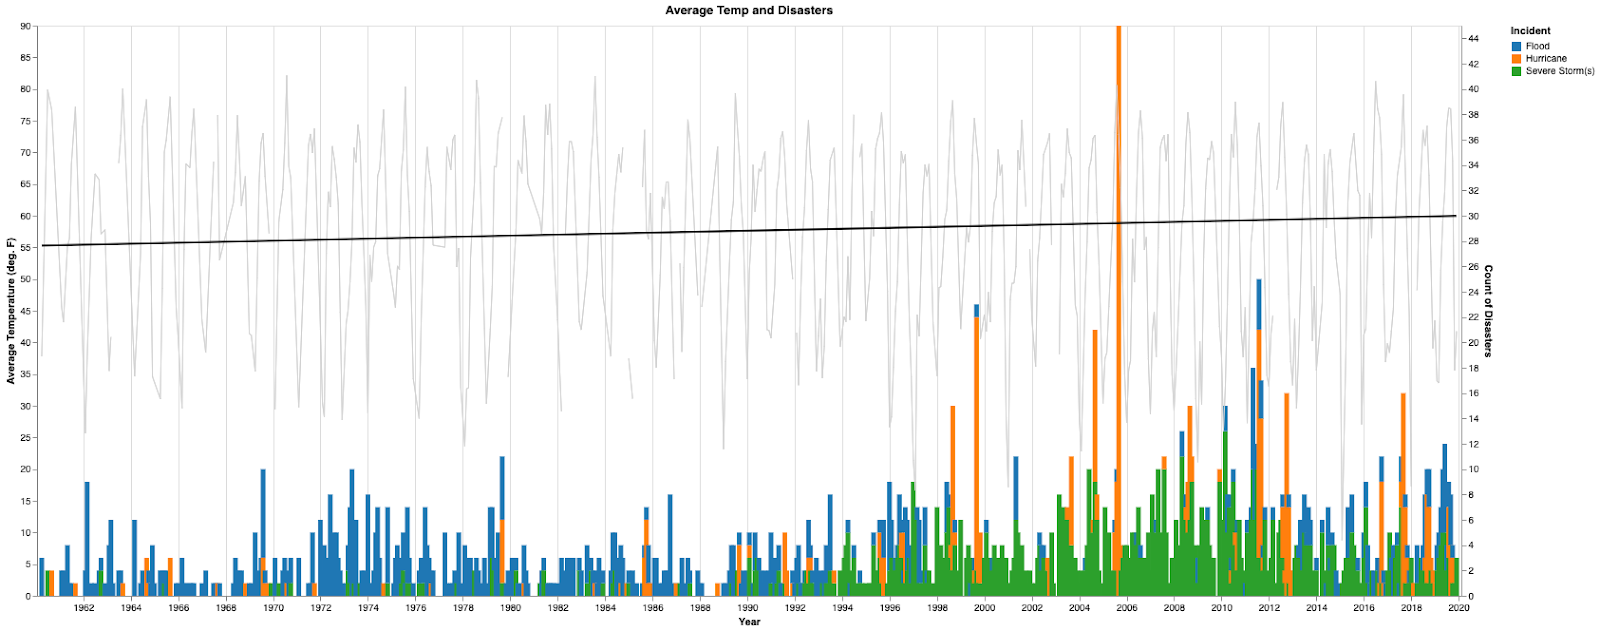
\includegraphics[scale=0.3]{iter2_h1.png}
    \caption{Hypothesis 1 - Iteration 2}
    \label{fig:my_label}
\end{figure}

\subsubsection*{What is Informative About This View?}
This view cleans up the amount of incidents shown, which reduces the cognitive load on the viewer. There are now only 3 incident types included in the visualization: floods, hurricanes, and severe storms. The linear regression line remains in order to show that there has been a gradual increase in average temperature over the years.

\subsubsection*{What Could Be Improved About This View?}
Including the minimum and maximum temperatures in addition to the average temperature may provide more context in understanding how temperature changes may have an effect on hurricane frequency. If I were to make updates to the viz, I would try to split the chart so that there is only one y-axis. In my mind, it made sense to include everything in one plot, but it could be confusing for others.

\subsection*{Conclusion}
 (do the data appear to support the hypothesis, or not?): These data views suggest that there have been an increase in hurricanes and severe storms. In 2005 there was a huge spike in hurricanes, which occurred when the average temperature for that year was at its peak. 
 
\section*{Hypothesis 2}
In the Southeastern US, severe storms and hurricanes become more frequent than any other type of FEMA declared disaster from 1960 - 2000. 

\subsection*{Iteration 1}
\begin{figure}[h]
    \centering
    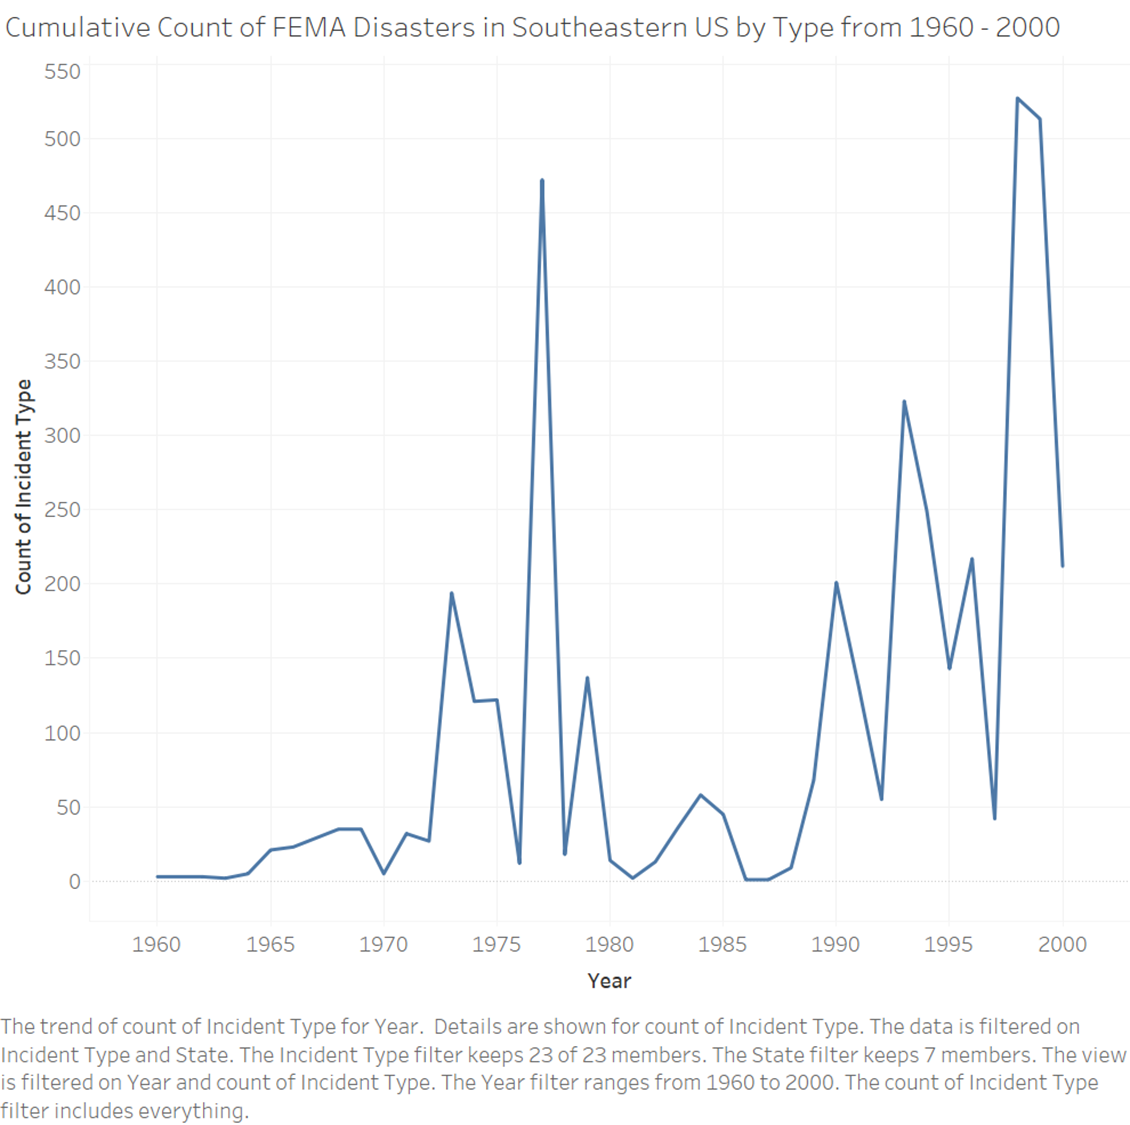
\includegraphics[scale=0.20]{iter1_h2.png}
    \caption{Hypothesis 2 - Iteration 1}
    \label{fig:my_label}
\end{figure}
\subsubsection*{What is Informative About This View?}
 Figure 3 shows the cumulative count of FEMA disasters in the Southeastern US (i.e., Tennessee, North Carolina, South Carolina, Mississippi, Alabama, Georgia, Florida). While it does not inform the audience of the breakdown of severe storms and hurricanes, it does show how the mid-late 1990s saw an increase in total disasters which is worth further exploration. 
 \subsubsection*{What Could Be Improved About This View?}
This view needs a breakdown of FEMA disasters for the audience to understand how each disaster type has changed over time. 
 \subsection*{Iteration 2}
\begin{figure}[h]
    \centering
    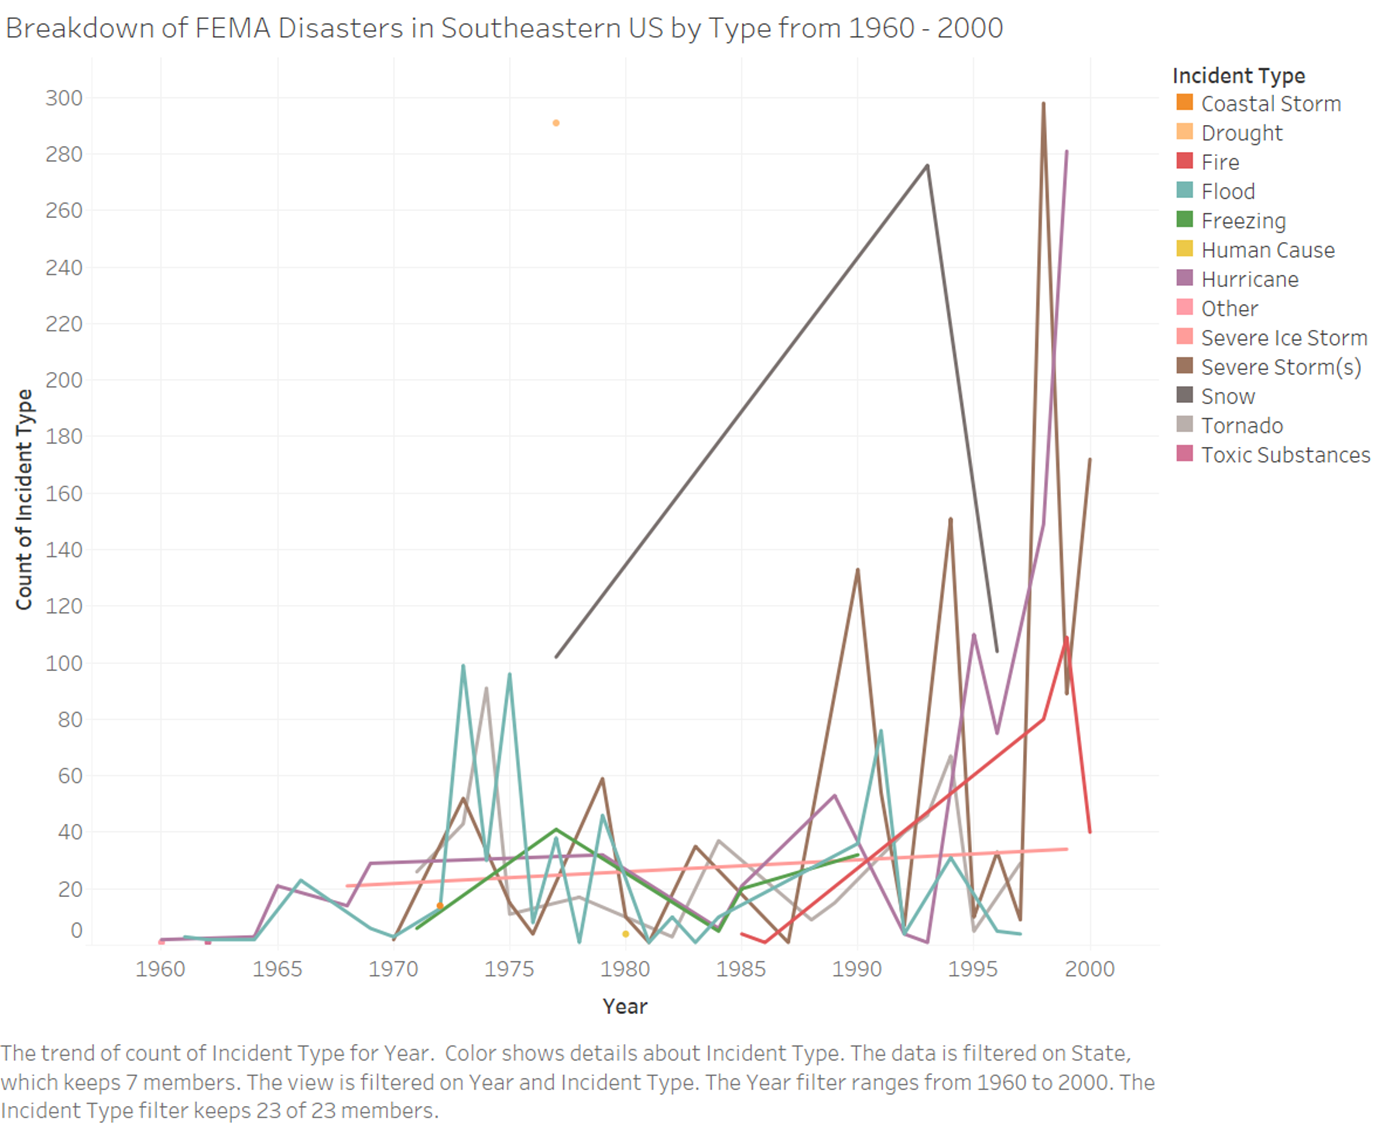
\includegraphics[scale=0.20]{iter2_h2.png}
    \caption{Hypothesis 2 - Iteration 2}
    \label{fig:my_label}
\end{figure}
\subsubsection*{What is Informative About This View?}
 Figure 4 depicts each FEMA disaster type and plots their counts by year. As we get closer to the later 1990s it becomes evident that hurricanes, severe storms and fires begin to rise in frequency. 
 \subsubsection*{What Could Be Improved About This View?}
 While informative, this chart can be unclear given the obfuscation caused by the overlapping plots. To provide greater clarity and reduce the cognitive load on the audience, another chart type should be explored.  
 
 \subsection*{Iteration 3}
 \begin{figure}[h]
    \centering
    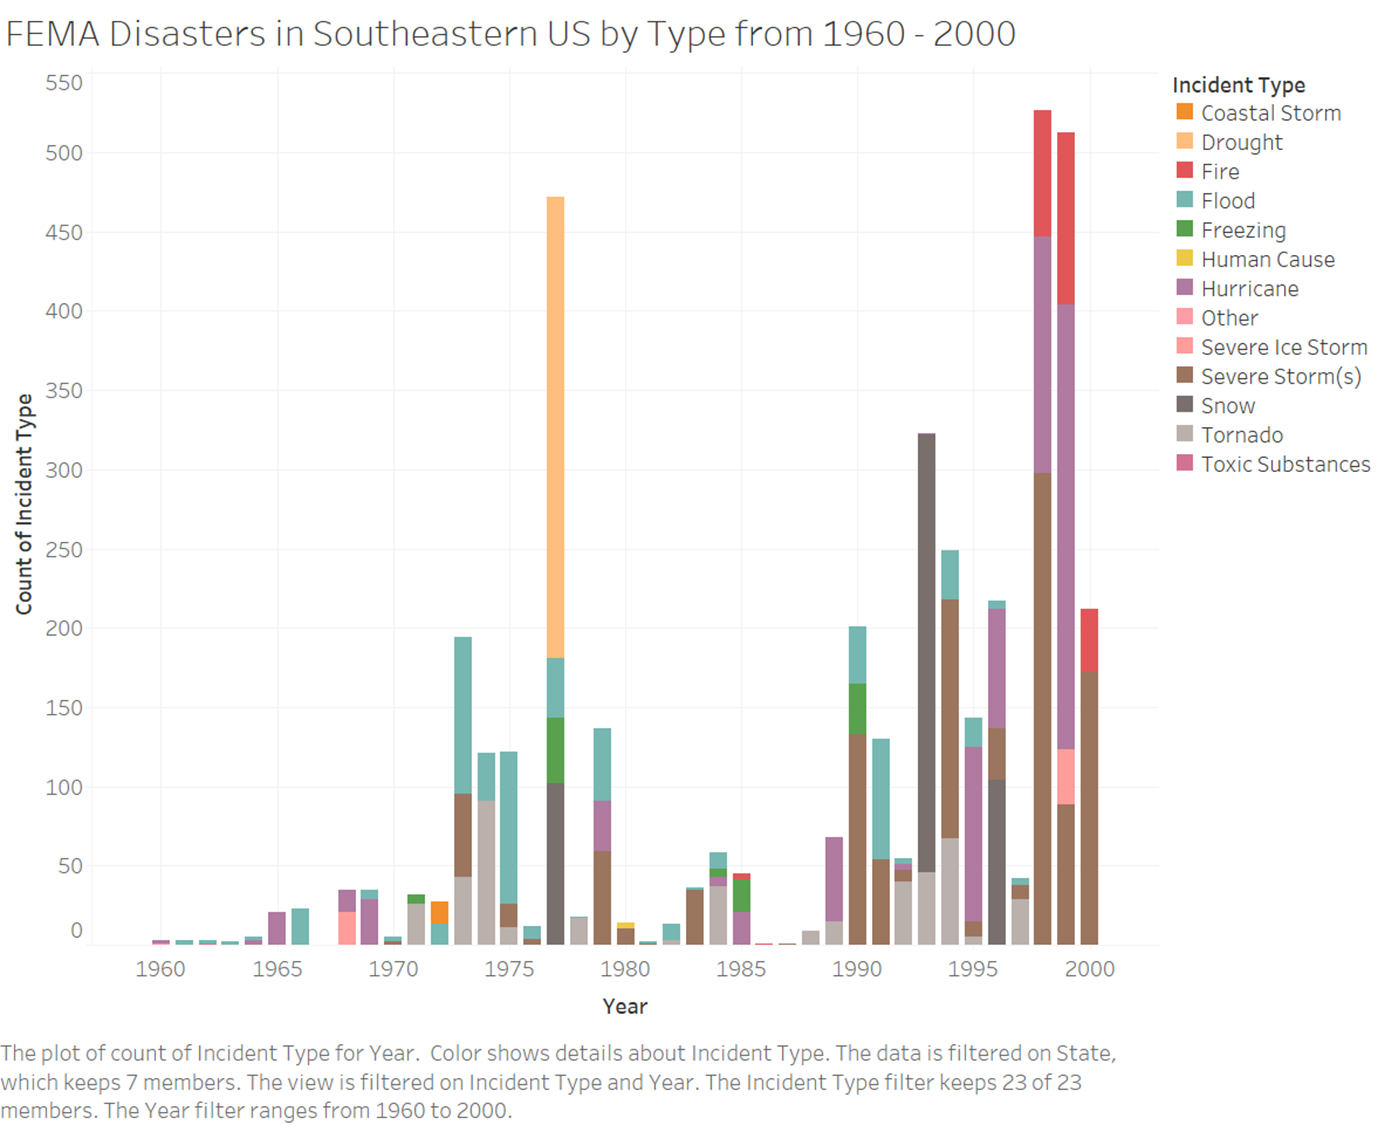
\includegraphics[scale=0.20]{iter3_h2.png}
    \caption{Hypothesis 2 - Iteration 2}
    \label{fig:my_label}
\end{figure}
\subsubsection*{What is Informative About This View?}
Figure 5 depicts each FEMA disaster type and plots their counts by year via a stacked bar chart. This view clearly shows the proportion of each incident to the overall count. From this chart, it’s evident that severe storms and hurricanes make up a majority of FEMA disasters in the late 1990s. 
\subsubsection*{What Could Be Improved About This View?}
 It would be useful to give the audience a way to interact with this chart in order to yield greater insight. For instance, the audience could be given the ability to filter certain incidents, choose different regions in the US or obtain the percentage change by year of a given disaster. 
\subsubsection*{Conclusion}
The evidence provided by this visualization supports the hypothesis that in the Southeastern US, severe storms and hurricanes become more frequent than any other type of FEMA declared disaster from 1960 - 2000.
  
\section*{Hypothesis 4}
Different parts of the United States are affected by different disasters more than other parts.

 \subsection*{Iteration 1}
 \begin{figure}[h]
    \centering
    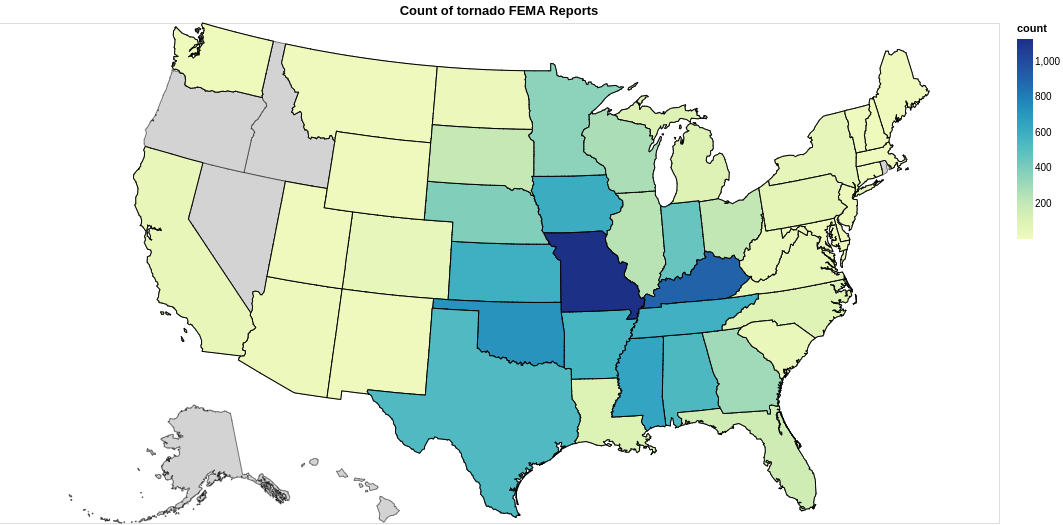
\includegraphics[scale=0.4]{iter1.0_h4.png}
    \caption{Hypothesis 4 - Iteration 1.0}
    \label{fig:my_label}
\end{figure}

\subsubsection*{What is Informative About This View?}
This view is dynamic, users can put in keywords and see where the reports pertaining to that specific keyword come from. This is informative because it clearly shows that there are certain parts of the country that are disproportionately affected by certain types of natural disasters. For example, the last figure shows the total occurrences of tornado reports by state - and we see that most of the reports come from the midwest. If we consider hurricane reports, we get the following. This clearly shows that most hurricane reports come from the southeastern part of the country - which is what we expect based on the geography and the proximity of that region to the gulf of mexico.

 \begin{figure}[h]
    \centering
    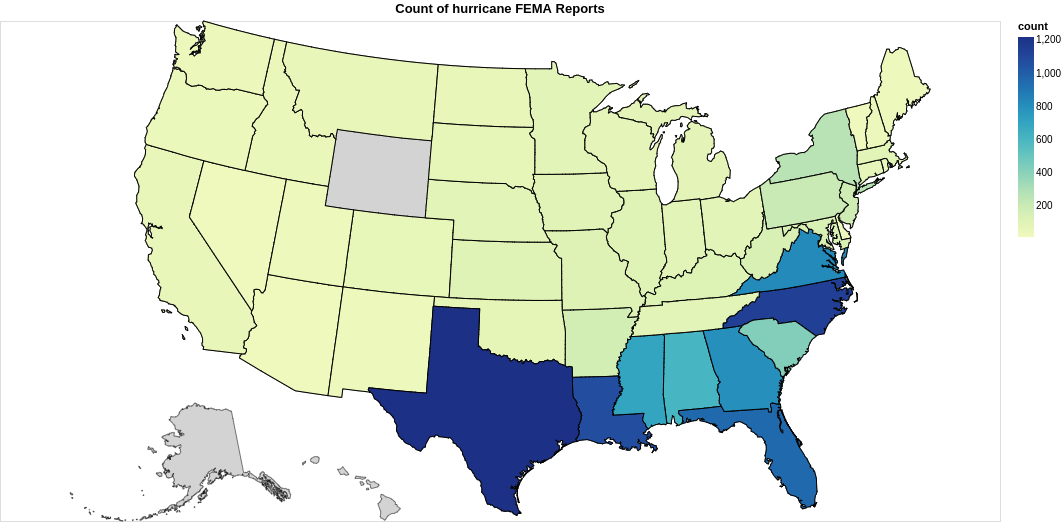
\includegraphics[scale=0.4]{iter1.1_h4.png}
    \caption{Hypothesis 4 - Iteration 1.1}
    \label{fig:my_label}
\end{figure}

We can also look at FEMA reports for blizzards, resulting in the following map:

 \begin{figure}[h]
    \centering
    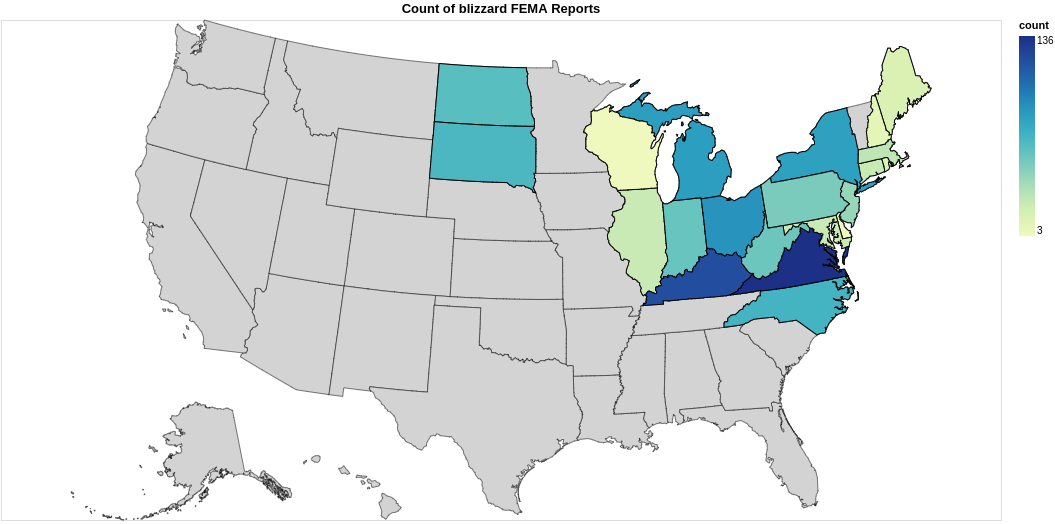
\includegraphics[scale=0.4]{iter1.2_h4.png}
    \caption{Hypothesis 4 - Iteration 1.2}
    \label{fig:my_label}
\end{figure}

\subsubsection*{What Could Be Improved About This View?}
 I’d like to work on the colors some more. This does not seem like an ideal color scheme to show the differences between the different quantities represented by count of FEMA reports out of the states. It would also be more legible if the lines separating the states were wider and also in a lighter color.
 
\subsection*{Iteration 2}
 
 \begin{figure}[h]
    \centering
    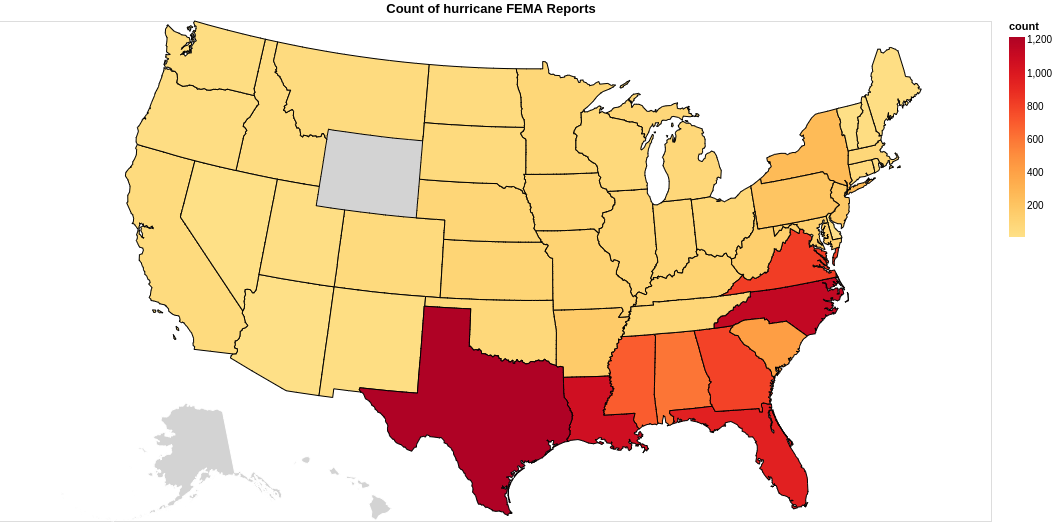
\includegraphics[scale=0.4]{iter2_h4.png}
    \caption{Hypothesis 4 - Iteration 2}
    \label{fig:my_label}
\end{figure}

\subsubsection*{What is Informative About This View?}
Using a different color scheme gives some more contrast between the values. The usefulness of the graphic, however, comes mainly from the interactive aspect of it - allowing users to search for certain disasters and get the count by state in order to see which areas of the United States are disproportionately affected by natural disasters, or not equipped to deal with them.

\subsubsection*{What Could Be Improved About This View?}
 This view would be more useful with a little bit more interactivity. Letting users filter by certain natural disasters is very useful, but having tooltips would make this a bit more useful.

\subsubsection*{Conclusion}
This visualization provides strong evidence that different natural disasters are more likely to occur in different parts of the United States.

\end{document}

